% !TEX root =  main.tex



\chapter{Introduction}
\label{chap:introduction}
\pagestyle{plain}
\setcounter{page}{1}

In the modern digital world, large and diverse data are being constantly generated. To manage this influx, organizations often scale horizontally, distributing data across multiple servers. This distribution of datasets however makes it difficult to discover and search for datasets. Current data management solutions like CKAN or Socrata \cite{datasetSearchSurvey} primarily rely on keyword and metadata filters such as file type and creation date to perform dataset search, which are contingent on the quality and availability of those metadata. Furthermore, we are interested in searching data for augmentation purpose: given a relational dataset, we want to identify which other datasets out there can be joined or unioned with one or more attributes from our query dataset. With limited search capability of such traditional dataset search systems, this task is often challenging, as humans are required in the process to perform specific keywords, and tediously sift through datasets to determine if there are any matching attribute in it. Therefore, a faster and automated approach is needed.

To illustrate the problem, consider figure \ref{fig:sendA}, which depicts a cluster with three nodes, each containing a number of datasets. Node N1 possesses dataset A, and wants to find out which datasets from node N2 and N3 can be joined with A. A naive approach would involve sending dataset A to nodes N2 and N3, requesting them to perform joins with each of their respective datasets. Firstly, this would incur a lot of traffic in the network, since dataset size can range anywhere from megabytes to gigabytes. Moreover, the feasibility of this method diminishes with an increasing number of nodes within the cluster. Secondly, once the dataset arrives in N2 and N3, how can they manage to perform join between A and all other datasets they have? And how do they decide that a join between an attribute in A and an attribute in another dataset is a reasonable join? (figure \ref{fig:exampleJoin}).

\begin{figure}
    \centering
    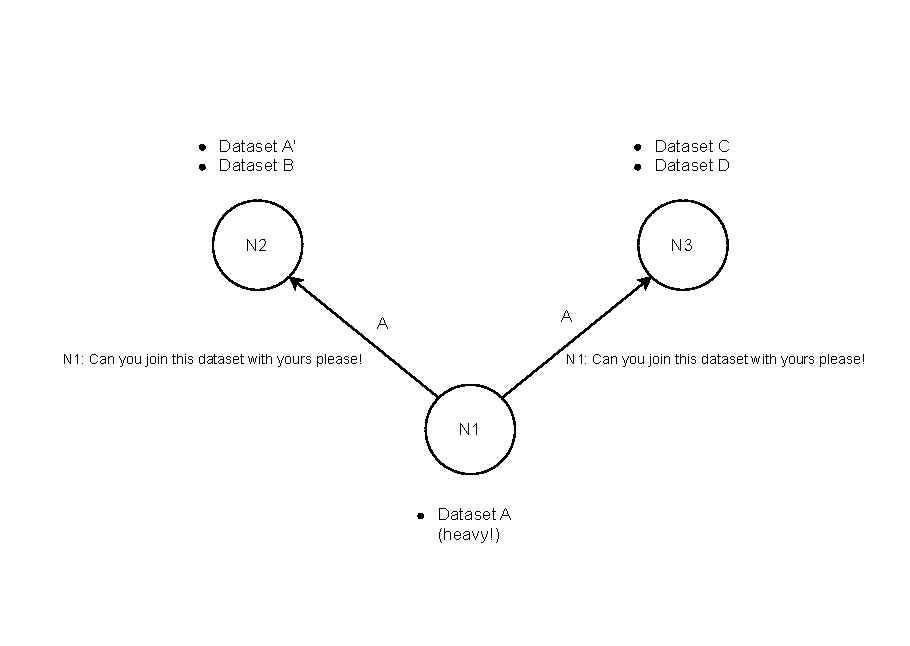
\includegraphics[width=\textwidth]{send A.pdf}
    \caption{A cluster of three nodes, N1 is attempting to send dataset A over the network}
    \label{fig:sendA}
\end{figure}

\begin{figure}
    \centering
    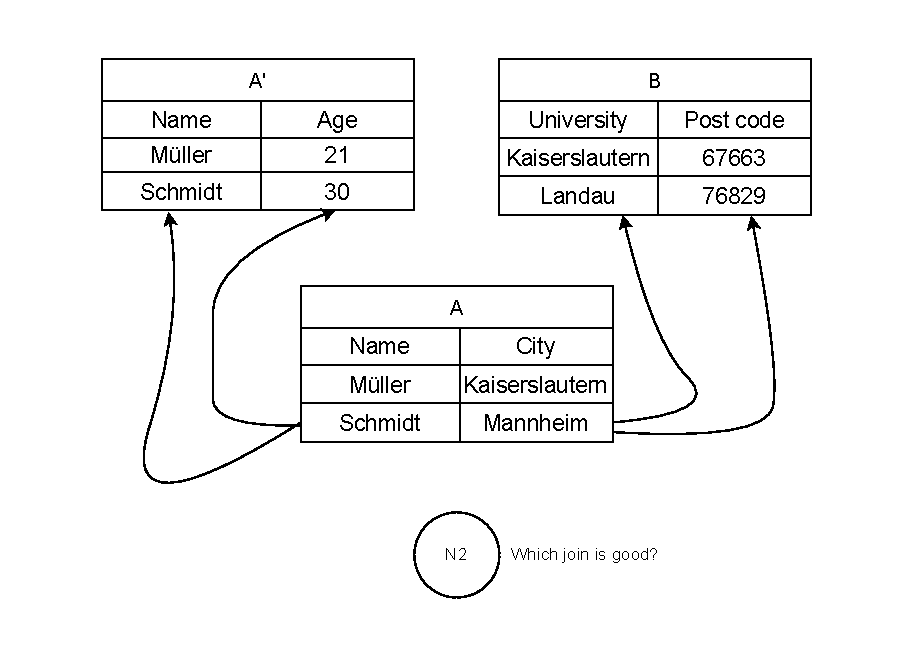
\includegraphics[width=\textwidth]{example join.pdf}
    \caption{Caption}
    \label{fig:exampleJoin}
\end{figure}

The goal of our work is to find a way to answer these questions. During research, we discovered that the task of searching for related datasets bears a lot of resemblance with the task of schema matching: finding semantic mapping between two schemas. Therefore, we apply schema matching techniques in our solution to help efficiently discover joinable and unionable attributes. Then, to accelerate the schema matching process and minimize network traffic, we employ a modern implementation of MinHash sketching and locality sensitive hashing (LSH) indexing.

The structure of the thesis is as following: chapter \ref{chap:background} supplies background knowledge on the topics of schema matching, its techniques, MinHash sketch, locality sensitive hashing, and REST API. Chapter \ref{chap:relatedwork} introduces other works that are related to or is the base of our implementation. Chapter \ref{chap:overview} presents an overview of the architecture of our system and the schema matching techniques used. In chapter \ref{chap:implementation}, we provide a detailed implementation of the system and an algorithm to optimize the search speed. Chapter \ref{chap:experimentalevaluation} carries out an empirical evaluation of the system's performance. Finally, the thesis ends with the conclusion, limitations and future work.





